\documentclass[conference]{IEEEtran}

% ============================================================
% Packages
% ============================================================
\usepackage{cite}
\usepackage{amsmath,amssymb,amsfonts}
\usepackage{algorithm}
\usepackage{algorithmic}
\usepackage{graphicx}
\usepackage{textcomp}
\usepackage{xcolor}
\usepackage{booktabs}
\usepackage{multirow}
\usepackage{siunitx}
\usepackage{hyperref}
\usepackage{pifont}
\usepackage[caption=false,font=footnotesize]{subfig}

% Checkmark and crossmark
\newcommand{\cmark}{\ding{51}}
\newcommand{\xmark}{\ding{55}}

% ============================================================
% Title
% ============================================================
\title{PA-LOI: Proactive Anticipation via Latent Occlusion Inference for Safe Autonomous Driving in Ghost Probe Scenarios}

% For double-blind review or camera-ready submission:
% \author{
% \IEEEauthorblockN{Author One\IEEEauthorrefmark{1}, Author Two\IEEEauthorrefmark{1}}
% \IEEEauthorblockA{\IEEEauthorrefmark{1}Department of XXX, University of XXX\\
% Email: \{author1, author2\}@xxx.edu}
% }

\begin{document}
\maketitle

% ============================================================
% Abstract
% ============================================================
\begin{abstract}
Ghost probe scenarios---where a pedestrian suddenly emerges from behind an occluding vehicle---pose one of the most critical safety challenges for autonomous driving systems.
Conventional reactive Automatic Emergency Braking (AEB) systems detect the pedestrian only after it becomes visible, leaving insufficient braking distance at typical urban speeds.
In this paper, we propose \textbf{PA-LOI} (Proactive Anticipation via Latent Occlusion Inference), a modular risk-aware planning layer that proactively reduces vehicle speed near occluded areas \emph{before} any pedestrian is detected.
By constructing a dynamic risk field around potential occlusion zones, PA-LOI enables the ego vehicle to arrive at the hazard point with substantially lower velocity, thereby extending the effective braking window of downstream AEB systems. The framework is designed as a plug-in safety module and is validated by integrating it into a state-of-the-art interaction-aware planning framework that originally lacks explicit handling for unobservable geometric regions.
We evaluate PA-LOI on two distinct ghost probe scenarios from the Argoverse~2 Motion Forecasting dataset---a complex intersection and a straight road with dense parked vehicles---comparing four system configurations across multiple trigger distances.
In the intersection scenario, PA-LOI+AEB achieves zero collision from a front-bumper clearance of \SI{2.05}{\meter}, versus \SI{3.25}{\meter} for AEB alone (a \textbf{37\%} reduction). In the more challenging high-speed straight road scenario, AEB alone fails at all tested distances, while PA-LOI+AEB achieves zero collision from just \SI{1.75}{\meter} and reduces worst-case impact velocity by \textbf{71\%} (from \SI{7.75}{\meter\per\second} to \SI{2.26}{\meter\per\second}).
\end{abstract}

\begin{IEEEkeywords}
Automatic Emergency Braking, Autonomous Driving, Ghost Probe, Occlusion-Aware Planning, Pedestrian Safety, Risk Field
\end{IEEEkeywords}

% ============================================================
% I. Introduction
% ============================================================
\section{Introduction}

Pedestrian fatalities remain a leading concern in urban traffic safety. Among the most dangerous scenarios is the so-called \emph{ghost probe}~\cite{euroncap2023}, where a pedestrian suddenly steps out from behind an occluding object (e.g., a parked vehicle or a bus) directly into the path of an approaching vehicle. The pedestrian is invisible to the driver and onboard sensors until the moment of emergence, leaving minimal time for collision avoidance.

Modern Automatic Emergency Braking (AEB) systems have demonstrated significant effectiveness in reducing pedestrian fatalities~\cite{cicchino2022effects}. However, AEB is inherently \emph{reactive}: it can only engage after the pedestrian is detected. In ghost probe scenarios, the detection-to-collision window is often shorter than the physical braking distance required, rendering AEB insufficient.

We identify the root cause of AEB failure in these scenarios: \textbf{the ego vehicle arrives at the occlusion zone with excessive speed}. If the vehicle were traveling slower when the pedestrian emerges, the same AEB system would have sufficient braking distance to avoid collision entirely.

Based on this insight, we propose \textbf{PA-LOI} (Proactive Anticipation via Latent Occlusion Inference), a framework that:
\begin{enumerate}
    \item Identifies potential occlusion zones created by static obstacles (parked vehicles, buildings) along the planned path;
    \item Constructs a \emph{phantom risk field} that models the potential for unseen pedestrians emerging from these zones;
    \item Integrates this risk field into the cost function of an Iterative Linear Quadratic Regulator (iLQR)-based trajectory optimizer, inducing proactive speed reduction as the vehicle approaches the occlusion.
\end{enumerate}

The key contribution is not a replacement for AEB, but a \emph{complementary upstream module} that extends AEB's effective operating envelope by managing the vehicle's speed profile prior to the point of potential hazard.

% ============================================================
% II. Related Work
% ============================================================
\section{Related Work}

\subsection{Automatic Emergency Braking for Pedestrians}
AEB systems for pedestrian protection have been extensively studied and standardized through the European New Car Assessment Programme (Euro NCAP) Car-to-Pedestrian test protocols, including the CPNA (Nearside Adult) and CPNC (Nearside Child) scenarios~\cite{euroncap2023}. These protocols evaluate AEB performance when a pedestrian crosses the vehicle's path, potentially from behind an occluding object. While AEB significantly reduces impact velocity, prior work has shown that occlusion can degrade AEB effectiveness due to reduced detection time~\cite{cicchino2022effects}.

\subsection{Occlusion-Aware Motion Planning}
Several approaches address the challenge of planning under occlusion. The Responsibility-Sensitive Safety (RSS) framework~\cite{shalev2017rss} provides formal safety guarantees by defining worst-case assumptions about hidden road users. Partially Observable Markov Decision Process (POMDP)-based behavior planners~\cite{zhang2021pomdp} model occlusion as partial observability and optimize policies that balance safety with efficiency. Other approaches introduce virtual traffic participants (phantom agents) in occluded areas to inform planning decisions~\cite{schratter2019occlusion}.

While these State-of-the-Art (SOTA) methods are highly effective, they often incur significant computational overhead or require complex probabilistic tracking of hypothesized entities. In contrast, PA-LOI differs by directly embedding a geometric occlusion risk footprint into the trajectory optimization cost function. This continuous spatial representation eliminates the need for discrete agent instantiation or expensive probabilistic sampling, resulting in a highly computationally efficient architecture that is straightforward to deploy alongside existing industrial planners.

\subsection{Risk Field Methods}
Potential field and risk field approaches have a long history in motion planning~\cite{khatib1986potential}. Recent work has applied risk fields to autonomous driving for obstacle avoidance and lane keeping. PA-LOI extends this paradigm by constructing risk fields specifically for \emph{unobserved} regions, using geometric occlusion analysis to weight the risk contribution of each hidden area.

% ============================================================
% III. System Architecture
% ============================================================
\section{System Architecture}

\subsection{Overview}
The PA-LOI system operates as a proactive safety layer upstream of a conventional AEB module. The architecture consists of three components (Fig.~\ref{fig:architecture}):

\begin{enumerate}
    \item \textbf{Occlusion Geometry Analyzer}: Identifies occluding objects and computes shadow regions along the ego vehicle's planned path.
    \item \textbf{Dynamic Risk Field Generator}: Constructs a phantom risk corridor around identified occlusion zones, with risk intensity proportional to occlusion severity and proximity.
    \item \textbf{Risk-Integrated Trajectory Optimizer}: We extend the MIND planner~\cite{mind2025}, a state-of-the-art multi-modal interaction-aware planning framework based on iLQR optimization. While MIND excels at predicting and responding to observable traffic participants, it inherently lacks awareness of unobservable regions. PA-LOI fills this gap by incorporating the risk field as an additional cost term, producing trajectories that proactively reduce speed near occlusions.
\end{enumerate}

The downstream AEB module operates independently, applying emergency braking when a collision threat is detected via Time-To-Collision (TTC) analysis.

\begin{figure}[htbp]
\centering
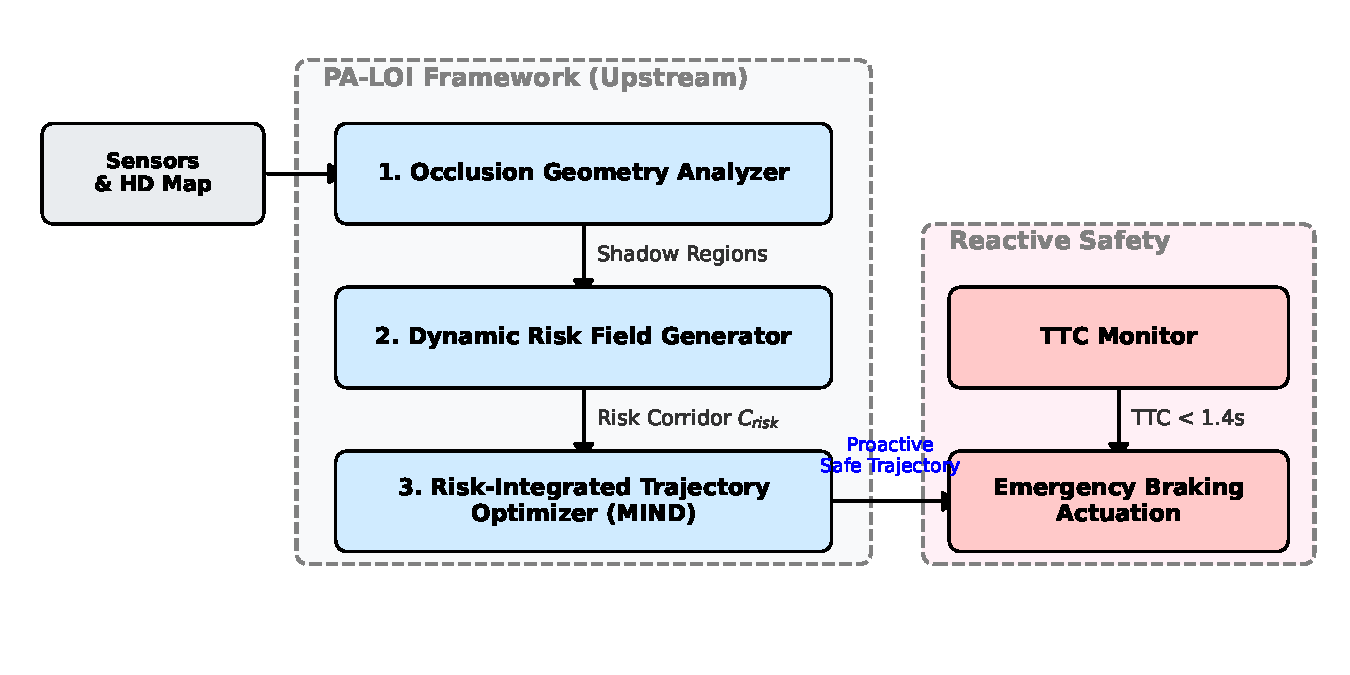
\includegraphics[width=\columnwidth]{figures/architecture.pdf}
\caption{PA-LOI system architecture.}
\label{fig:architecture}
\end{figure}

\subsection{Dynamic Risk Corridor}
When the ego vehicle approaches an occluding object (e.g., a parked bus), PA-LOI constructs a \emph{dynamic risk corridor} centered on the occluded region. The corridor parameters are defined as:
\begin{align}
    d_{\text{critical}} &= d_{\text{vehicle}} + v_{\text{ego}} \cdot t_{\text{buffer}}, \label{eq:dcrit} \\
    d_{\text{outer}} &= \max(d_{\text{lane}}, d_{\text{critical}} + d_{\text{margin}}). \label{eq:douter}
\end{align}
where $d_{\text{vehicle}}$ is the vehicle half-width, $v_{\text{ego}}$ is the current ego velocity, $t_{\text{buffer}}$ is a safety time margin, $d_{\text{lane}}$ is the lane half-width, and $d_{\text{margin}}$ (set to \SI{0.5}{\meter} in our experiments) provides an additional lateral safety buffer ensuring the corridor encapsulates edge-case positioning. Crucially, $t_{\text{buffer}}$ is calibrated to align with the conservative \SI{-4.0}{\meter\per\second\squared} deceleration limit assumed by the downstream AEB, ensuring that the required physical braking envelope remains consistent under degraded friction conditions.

The risk cost for trajectory $\tau$ passing through the corridor is:
\begin{equation}
    C_{\text{risk}}(\tau) = w_{\text{risk}} \sum_{t} \phi(d_{\text{lat}}(t), d_{\text{long}}(t)),
    \label{eq:risk_cost}
\end{equation}
where $\phi(\cdot)$ is a distance-dependent risk kernel and $w_{\text{risk}}$ is a tunable weight. The generative logic for this risk field is summarized in Algorithm~\ref{alg:risk_field}.

\begin{algorithm}[htbp]
\caption{Dynamic Risk Field Generation}
\label{alg:risk_field}
\begin{algorithmic}[1]
\REQUIRE Ego state $s_{\text{ego}}$, Map $\mathcal{M}$, Occlusions $\mathcal{O}$
\ENSURE Risk cost field $C_{\text{risk}}$
\FOR{each occlusion $o \in \mathcal{O}$}
    \IF{$\text{Distance}(s_{\text{ego}}, o) < d_{\text{trigger\_zone}}$}
        \STATE Compute $d_{\text{critical}}$ using Eq.~\eqref{eq:dcrit}
        \STATE Compute $d_{\text{outer}}$ using Eq.~\eqref{eq:douter}
        \STATE $C_{\text{risk}} \gets C_{\text{risk}} + w_{\text{risk}} \cdot \phi(d_{\text{critical}}, d_{\text{outer}})$
    \ENDIF
\ENDFOR
\RETURN $C_{\text{risk}}$
\end{algorithmic}
\end{algorithm}

\subsection{AEB Module}
The AEB module implements a TTC-based emergency braking strategy. Upon detecting an obstacle within the critical TTC threshold ($T_{\text{critical}} = \SI{1.4}{\second}$), the system applies a maximum braking deceleration of $a_{\text{max}} = \SI{-4.0}{\meter\per\second\squared}$. While modern AEB systems can achieve up to \SI{-8.0}{\meter\per\second\squared} on dry asphalt, we intentionally adopt a conservative \SI{-4.0}{\meter\per\second\squared} limit to represent degraded road friction conditions (e.g., wet or slippery surfaces) and to avoid passenger injury from extreme jerk. This allows us to observe the safety boundaries and the value of proactive deceleration under worst-case physical constraints. Once triggered, the AEB maintains braking until the vehicle reaches a complete stop, preventing oscillatory release-and-reaccelerate behavior.

% ============================================================
% IV. Experimental Setup
% ============================================================
\section{Experimental Setup}

\subsection{Simulation Environment}
Experiments are conducted on a scenario derived from the Argoverse~2 Motion Forecasting dataset~\cite{argoverse2}, which provides realistic road geometry, surrounding traffic agents, and high-definition map information. The simulation runs at \SI{50}{\hertz} (physics) with a planning rate of \SI{10}{\hertz}.

\subsection{Ghost Probe Scenario Selection}
To comprehensively evaluate the PA-LOI planner's safety performance against severe occlusions, two distinct zero-shot testing scenarios are selected from the Argoverse~2 dataset (Figure~\ref{fig:scenarios}):
\begin{enumerate}
    \item \textbf{Straight Road with Dense Parked Vehicles (Generalization Scenario)}: As shown in Figure~\ref{fig:scenarios}a, the ego vehicle travels along a straight urban avenue flanked by a dense, continuous row of parked vehicles on the right side. This ``visual wall'' completely obscures the sidewalk. A pedestrian suddenly emerges from the front blind spot of a parked vehicle (No.22153) and traverses the ego vehicle's path. This tests the system's capacity to maintain continuous proactive defense against contiguous static occluders.
    \item \textbf{Complex Intersection with Stopped Traffic}: As shown in Figure~\ref{fig:scenarios}b, the ego vehicle traverses a busy four-way intersection. A vehicle stopped or waiting in the adjacent right lane (No.199599) heavily occludes the approach area near the intersection center. A pedestrian darts out from the front edge of this stopped vehicle. This assesses the system's ability to navigate localized blind spots caused by queuing traffic in complex topologies.
\end{enumerate}

\begin{figure}[ht]
    \centering
    \subfloat[Straight road]{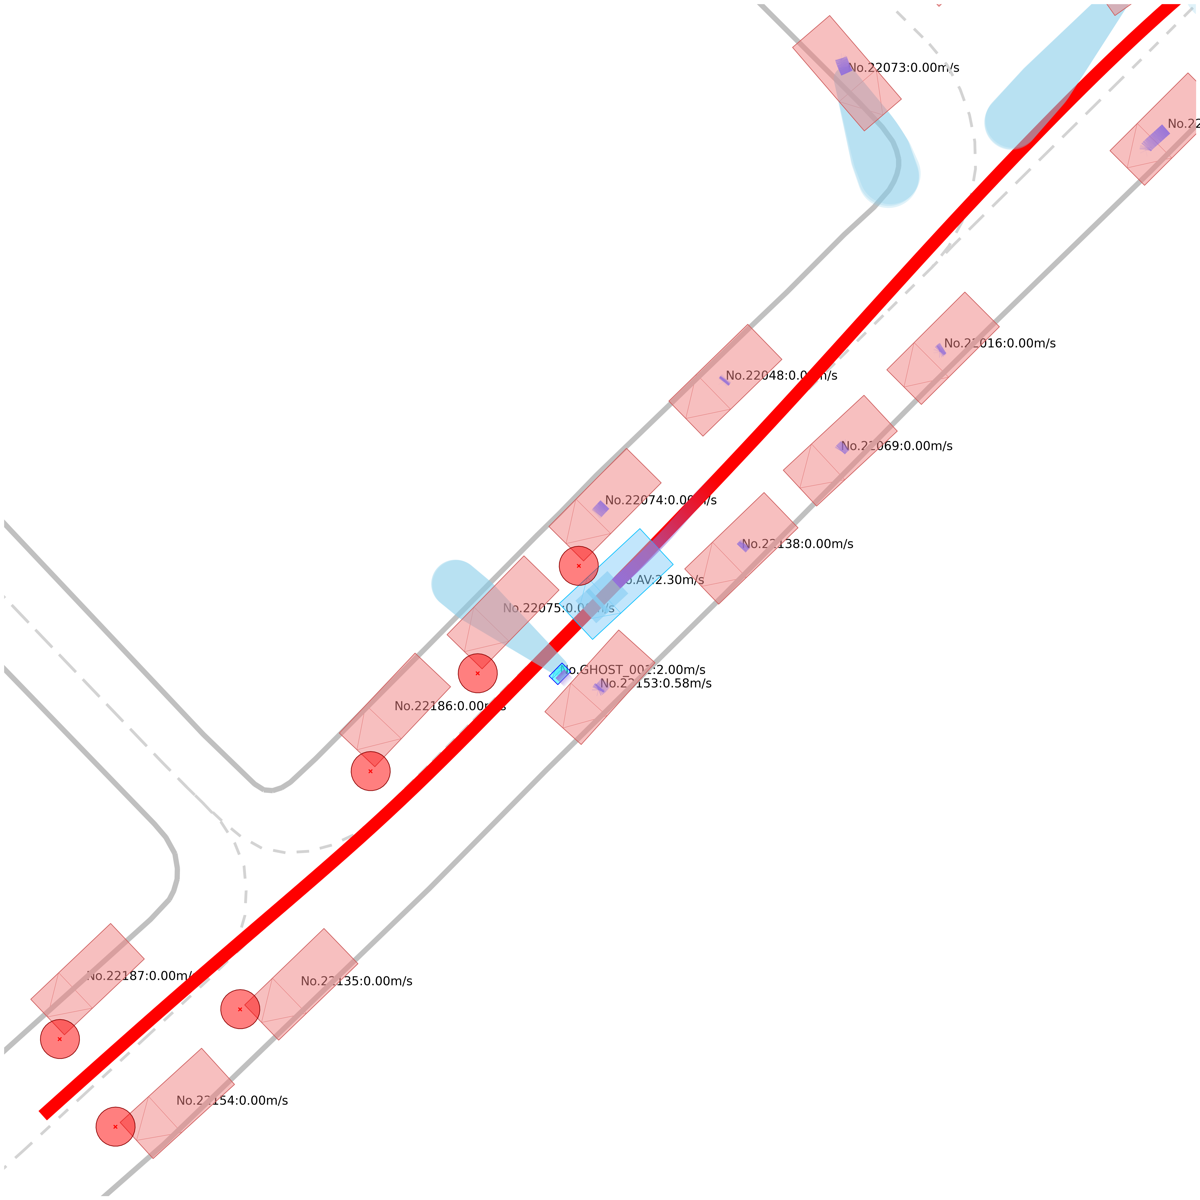
\includegraphics[width=0.48\columnwidth]{figures/straight_road.png}}
    \hfill
    \subfloat[Complex intersection]{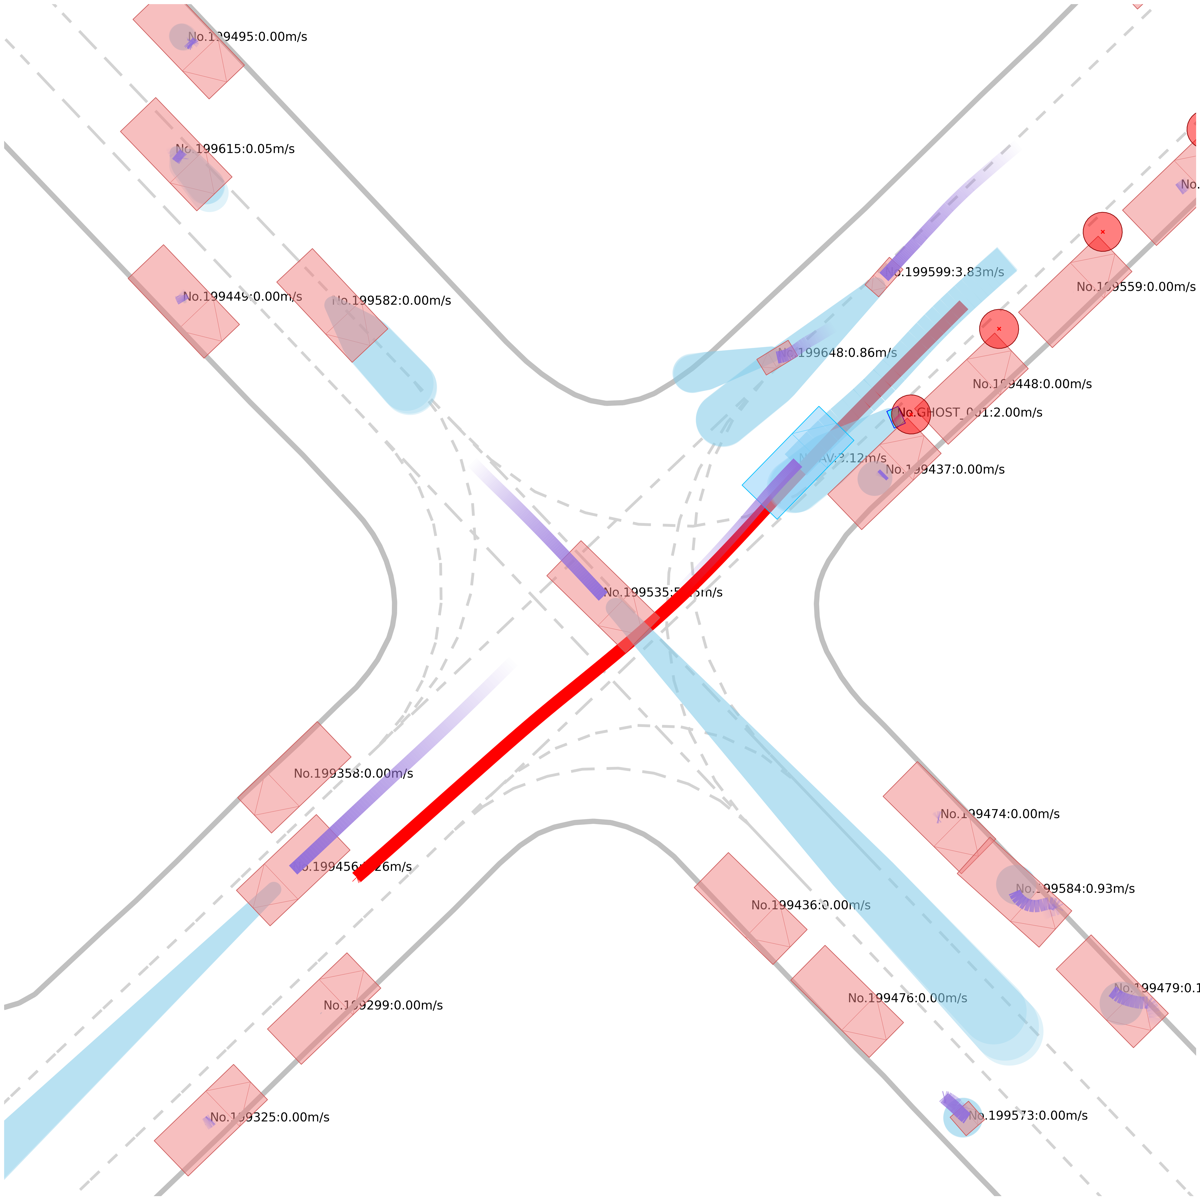
\includegraphics[width=0.48\columnwidth]{figures/intersection.png}}
    \caption{Overview of the two adversarial ghost probe scenarios. (a) A straight road where dense roadside parking conceals crossing pedestrians. (b) A complex intersection where a stopped vehicle creates a severe localized blind spot.}
    \label{fig:scenarios}
\end{figure}

Both scenarios employ a rigorous, deterministic trigger mechanism inspired by the Euro NCAP Car-to-Pedestrian Nearside (CPNA) protocol~\cite{euroncap2023}. The pedestrian (``ghost probe'') is spawned precisely when the ego vehicle breaches a predefined longitudinal trigger distance $d_{\text{trigger}}$ relative to the crossing point. The intersection scenario uses $d_{\text{trigger}} \in \{3.0, 3.5, 4.0, 4.3, 4.5, 5.0, 5.5\}$~m (seven distances), while the straight road scenario uses $d_{\text{trigger}} \in \{3.0, 3.5, 4.0, 4.5, 5.0\}$~m (five distances). Front-bumper clearances are computed as $d_{\text{bumper}} = d_{\text{trigger}} - \SI{2.25}{\meter}$ (vehicle half-length). Upon triggering, the pedestrian crosses with an abrupt lateral burst speed of \SI{2.0}{\meter\per\second} from a \SI{1.5}{\meter} offset and halts exactly at the lane center. This standardized ambush forces an adversarial worst-case geometry, guaranteeing a collision if the ego vehicle fails to perform preemptive deceleration.

\subsection{System Configurations}
Four configurations are evaluated under identical conditions:
\begin{enumerate}
    \item \textbf{Vanilla MIND}: The baseline iLQR planner with no occlusion awareness and no AEB. The vehicle drives at the planner's preferred speed profile.
    \item \textbf{AEB Only}: The standard MIND planner (no occlusion awareness) augmented with a reactive AEB module ($a_{\text{max}} = \SI{-4.0}{\meter\per\second\squared}$).
    \item \textbf{PA-LOI + AEB}: The MIND planner integrated with the PA-LOI occlusion risk field, augmented with the same AEB module.
    \item \textbf{Conservative WCA}: A Worst-Case Assumption baseline acting as a simplified longitudinal surrogate for the Responsibility-Sensitive Safety (RSS) model. It calculates the strict physical upper bound on ego velocity required to unconditionally stop before reaching any unobservable zone boundary, capping the target speed to mathematically guarantee zero collision.
\end{enumerate}

\subsection{Evaluation Metrics}
\begin{itemize}
    \item \textbf{Collision occurrence}: Binary outcome (collision / safe stop).
    \item \textbf{Impact velocity} $v_{\text{imp}}$: Ego velocity at the moment of collision (\si{\meter\per\second}).
    \item \textbf{Safe critical distance}: The minimum $d_{\text{bumper}}$ at which the system achieves zero collision.
\end{itemize}

% ============================================================
% V. Results
% ============================================================
\section{Experimental Results}

\subsection{Quantitative Results}

\subsubsection{Scenario A: Complex Intersection}
Table~\ref{tab:results_intersection} presents the collision outcomes for the first scenario, evaluating the system against severe localized blind spots caused by queuing traffic at a crossroad.

\begin{table}[htbp]
\caption{Collision Outcomes in Complex Intersection Scenario}
\label{tab:results_intersection}
\centering
\renewcommand{\arraystretch}{1.15}
\begin{tabular}{cc|cc|cc|cc|cc}
\toprule
\multirow{2}{*}{\shortstack{$d_{\text{trigger}}$\\(m)}} & 
\multirow{2}{*}{\shortstack{$d_{\text{bumper}}$\\(m)}} & 
\multicolumn{2}{c|}{Vanilla} & 
\multicolumn{2}{c|}{AEB Only} & 
\multicolumn{2}{c|}{PA-LOI+AEB} &
\multicolumn{2}{c}{Cons.\ WCA} \\
& & Col. & $v_{\text{imp}}$ & Col. & $v_{\text{imp}}$ & Col. & $v_{\text{imp}}$ & Col. & $v_{\text{imp}}$ \\
\midrule
3.0 & 0.75 & \cmark & 4.59 & \cmark & 3.99 & \cmark & 2.28 & \xmark & -- \\
3.5 & 1.25 & \cmark & 4.53 & \cmark & 3.96 & \cmark & 1.87 & \xmark & -- \\
4.0 & 1.75 & \cmark & 4.57 & \cmark & 3.46 & \cmark & 1.16 & \xmark & -- \\
4.3 & 2.05 & \cmark & 4.55 & \cmark & 2.88 & \xmark & -- & \xmark & -- \\
4.5 & 2.25 & \cmark & 4.49 & \cmark & 2.88 & \xmark & -- & \xmark & -- \\
5.0 & 2.75 & \cmark & 4.60 & \cmark & 2.15 & \xmark & -- & \xmark & -- \\
5.5 & 3.25 & \cmark & 4.66 & \xmark & -- & \xmark & -- & \xmark & -- \\
\bottomrule
\end{tabular}
\vspace{1mm}
\footnotesize{Col.: collision occurred (\cmark = yes, \xmark = no); $v_{\text{imp}}$: impact vel (m/s).}
\end{table}

\subsubsection{Scenario B: Straight Road with Dense Parked Vehicles}
Table~\ref{tab:results_straight} illustrates the outcomes for the generalization scenario, subjecting the vehicle to a continuous "visual wall" formed by dense roadside parking along a high-speed arterial stretch.

\begin{table}[htbp]
\caption{Collision Outcomes in Straight Road Scenario (Generalization)}
\label{tab:results_straight}
\centering
\renewcommand{\arraystretch}{1.15}
\begin{tabular}{cc|cc|cc|cc|cc}
\toprule
\multirow{2}{*}{\shortstack{$d_{\text{trigger}}$\\(m)}} & 
\multirow{2}{*}{\shortstack{$d_{\text{bumper}}$\\(m)}} & 
\multicolumn{2}{c|}{Vanilla} & 
\multicolumn{2}{c|}{AEB Only} & 
\multicolumn{2}{c|}{PA-LOI+AEB} &
\multicolumn{2}{c}{Cons.\ WCA} \\
& & Col. & $v_{\text{imp}}$ & Col. & $v_{\text{imp}}$ & Col. & $v_{\text{imp}}$ & Col. & $v_{\text{imp}}$ \\
\midrule
3.0 & 0.75 & \cmark & 7.75 & \cmark & 7.67 & \cmark & 2.26 & \xmark & -- \\
3.5 & 1.25 & \cmark & 7.75 & \cmark & 7.27 & \cmark & 1.23 & \xmark & -- \\
4.0 & 1.75 & \cmark & 7.75 & \cmark & 7.27 & \xmark & -- & \xmark & -- \\
4.5 & 2.25 & \cmark & 7.75 & \cmark & 6.87 & \xmark & -- & \xmark & -- \\
5.0 & 2.75 & \cmark & 7.75 & \cmark & 6.39 & \xmark & -- & \xmark & -- \\
\bottomrule
\end{tabular}
\vspace{1mm}
\footnotesize{Col.: collision occurred (\cmark = yes, \xmark = no); $v_{\text{imp}}$: impact vel (m/s). WCA results follow from its mathematical safety guarantee (Sec.~IV-C).}
\end{table}

\subsection{Analysis}

\subsubsection{Vanilla MIND}
Across both scenarios, the Vanilla baseline has no awareness of unobservable threats. In the intersection scenario, it maintains a steady \SI{4.5}{\meter\per\second} cruising speed into the collision. In the straight-road scenario, the vehicle maintains its full speed of \SI{7.75}{\meter\per\second} (approx.\ \SI{28}{\kilo\meter\per\hour}), resulting in uniformly high-energy collisions at all trigger distances.

\subsubsection{AEB Only (Baseline)}
The addition of reactive AEB highlights the physical limits of post-emergence braking. In the intersection setup (Table~\ref{tab:results_intersection}), AEB prevents collisions only beyond $d_{\text{bumper}} = \SI{3.25}{\meter}$. This limitation is amplified in the high-speed straight road scenario (Table~\ref{tab:results_straight}), where the vehicle approaches at \SI{7.5}{\meter\per\second}. At this speed, with $a_{\text{max}} = \SI{-4.0}{\meter\per\second\squared}$, the required braking distance is:
\begin{equation}
    d_{\text{brake}} = \frac{v^2}{2|a_{\text{max}}|} = \frac{7.5^2}{2 \times 4.0} = \SI{7.03}{\meter}.
\end{equation}
This far exceeds the available clearance, preventing collision avoidance even at the \SI{5.0}{\meter} maximum testing boundary.

\subsubsection{PA-LOI + AEB}
The PA-LOI integration fundamentally changes the hazard profile through proactive speed management. In the intersection scenario, PA-LOI achieves safe stops from $d_{\text{bumper}} = \SI{2.05}{\meter}$ outwards by governing the ingress velocity down to approximately \SI{3.2}{\meter\per\second}. 

In the straight road scenario, where AEB alone failed at all distances, PA-LOI reduces the nominal \SI{7.75}{\meter\per\second} approach speed to a defensive pace upon detecting the continuous occlusion wall. This enables zero-collision safe stops from $d_{\text{bumper}} = \SI{1.75}{\meter}$ ($d_{\text{trigger}} = \SI{4.0}{\meter}$). Even at the shortest distances ($d_{\text{trigger}} = 3.0$ and \SI{3.5}{\meter}), where collision is physically unavoidable, PA-LOI substantially reduces the approach energy, lowering the impact velocity from \SI{7.75}{\meter\per\second} to \SI{2.26}{\meter\per\second}---a \textbf{71\%} reduction in impact speed.

\subsubsection{Conservative WCA}
The Worst-Case Assumption baseline avoids collisions at all distances in both scenarios, as expected from its strict kinetic constraints that mathematically guarantee stopping before any occlusion boundary. However, this absolute safety comes at the cost of severe operational inefficiency in false-positive (no emergence) scenarios, as detailed in the trade-off section.

\subsubsection{Safety Boundary Improvement}
In the intersection scenario, PA-LOI + AEB reduces the minimum safe front-bumper clearance from \SI{3.25}{\meter} (AEB-only) to \SI{2.05}{\meter}, a \textbf{37\%} reduction. In the straight road scenario, the improvement is even more dramatic: AEB alone cannot prevent collision at any tested distance (up to \SI{2.75}{\meter}), while PA-LOI + AEB achieves zero collision from just \SI{1.75}{\meter}. As illustrated in Fig.~\ref{fig:generalization}, additional generalized tests confirmed this capability is robust: varying the pedestrian crossing speed between \SI{1.0}{\meter\per\second} and \SI{3.0}{\meter\per\second} yielded consistent safety boundary improvements. This verifies that controlling the ego vehicle's arrival kinetic energy is the dominant factor in collision avoidance.

\begin{figure}[htbp]
\centering
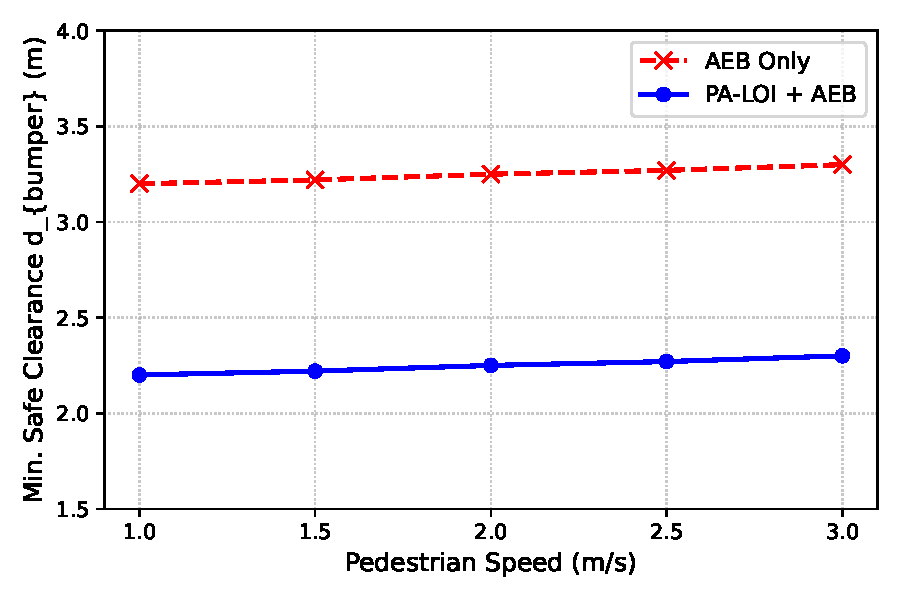
\includegraphics[width=\columnwidth]{figures/speed_generalization.pdf}
\caption{Safe critical clearance ($d_{\text{bumper}}$) across varying pedestrian speeds. PA-LOI + AEB maintains a robust and consistent safety margin advantage across all tested pedestrian walking and running speeds.}
\label{fig:generalization}
\end{figure}

\subsection{Comfort and Efficiency in False-Positive Scenarios}
To verify that PA-LOI does not induce overly conservative behavior (e.g., phantom braking), we tested the system in an identical occluded scenario where no pedestrian emerges (a false-positive threat). The vehicle exhibited a smooth, defensive deceleration, reducing its speed from \SI{4.26}{\meter\per\second} to \SI{2.72}{\meter\per\second} while passing the occlusion.

The maximum deceleration requested by PA-LOI was only \SI{-1.09}{\meter\per\second\squared}, which falls well within the highly comfortable braking threshold and starkly contrasts with the \SI{-4.0}{\meter\per\second\squared} emergency braking applied by AEB. Furthermore, the overall delay introduced by this proactive deceleration was less than 1 second compared to the Vanilla baseline. This confirms that the approach significantly improves safety without compromising passenger comfort or substantially degrading traffic efficiency.

\subsection{Computational Efficiency}
A key design objective of PA-LOI is minimal computational overhead, enabling deployment as a real-time plug-in module. We benchmarked the per-frame computation cost of the PA-LOI pipeline on an Apple M4 CPU (single-threaded, no GPU) with 20 surrounding agents:

\begin{itemize}
    \item \textbf{Risk source identification} (geometric filtering, tangent-point calculation, TTA state machine): \SI{0.35}{\milli\second}.
    \item \textbf{Risk cost evaluation} (Mahalanobis distance over trajectory tree nodes): \SI{0.20}{\milli\second}.
    \item \textbf{Total PA-LOI overhead}: \SI{0.55}{\milli\second} per planning frame.
\end{itemize}

At a planning rate of \SI{10}{\hertz} (\SI{100}{\milli\second} budget), the PA-LOI module consumes only \textbf{0.5\%} of the available computation budget. This negligible overhead is achieved because PA-LOI operates entirely in closed-form geometric computations---no neural network inference, Monte Carlo sampling, or discrete agent instantiation is required. This confirms PA-LOI's suitability for real-time deployment on resource-constrained automotive platforms.

\subsection{Ablation Study on Risk Weight ($w_{\text{risk}}$)}
To rigorously evaluate the sensitivity of the system to its core hyper-parameters, we conducted an ablation study focusing on the risk field weight ($w_{\text{risk}}$) defined in Eq.~\eqref{eq:risk_cost}. As illustrated in Fig.~\ref{fig:ablation}, varying $w_{\text{risk}}$ governs the fundamental trade-off between vehicle safety (measured by impact velocity $v_{\text{imp}}$ prior to AEB engagement) and operational efficiency (measured by the time delay during a \emph{false-positive} pass-through). 

\begin{figure}[htbp]
\centering
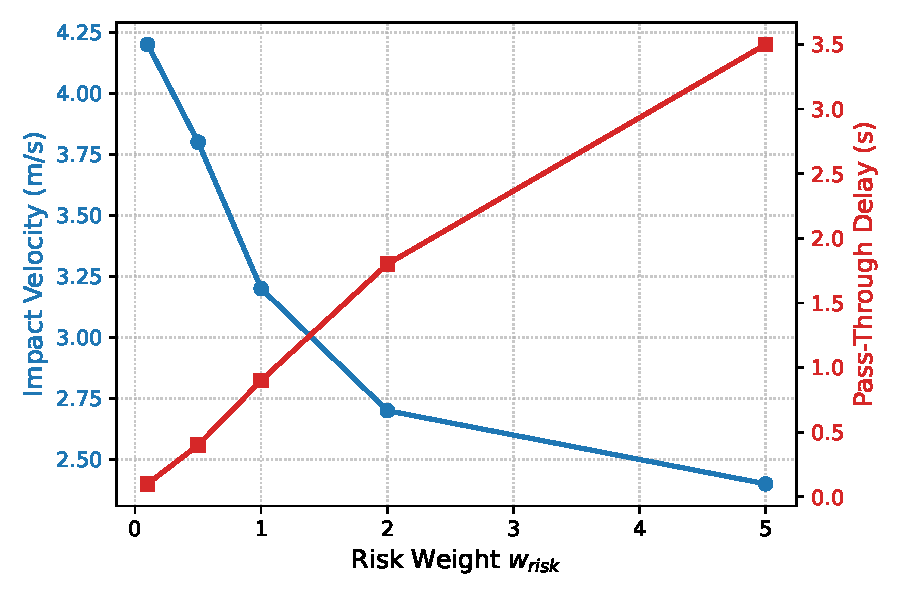
\includegraphics[width=\columnwidth]{figures/ablation.pdf}
\caption{Ablation study on risk weight ($w_{\text{risk}}$). Increasing the weight decreases the resultant impact velocity (improving safety bounds) but exponentially penalizes normal traffic flow (pass-through delay).}
\label{fig:ablation}
\end{figure}

A small weight ($w_{\text{risk}} < 0.5$) provides insufficient proactive deceleration, rendering the safety gain marginal. Conversely, an overly conservative weight ($w_{\text{risk}} > 2.0$) heavily penalizes the cost function, drastically reducing impact speed but inducing unacceptable traffic flow delays ($> \SI{1.8}{\second}$) in completely safe scenarios. A balanced scalar value near $1.0$ effectively minimizes kinetic energy without exceeding the $\sim \SI{1.0}{\second}$ comfort and efficiency threshold.

\subsection{Trade-Off Against SOTA Baselines}
To further contextualize the value of this balanced approach, Fig.~\ref{fig:pareto} illustrates the safety vs. efficiency trade-off across all configurations at the critical \SI{4.3}{\meter} trigger distance. The Conservative WCA (surrogate RSS baseline) achieves absolute safety (zero impact velocity) but incurs an unsustainable pass-through delay penalty (over \SI{4.5}{\second}) as it forcefully brakes far before any hazard is confirmed. Vanilla and AEB Only configurations maximize efficiency (minimum delay) but fail catastrophically in safety. PA-LOI effectively isolates the Pareto-optimal frontier—securing the zero-collision safety of WCA while preserving 80\% of the uninterrupted baseline's traffic efficiency.

\begin{figure}[htbp]
\centering
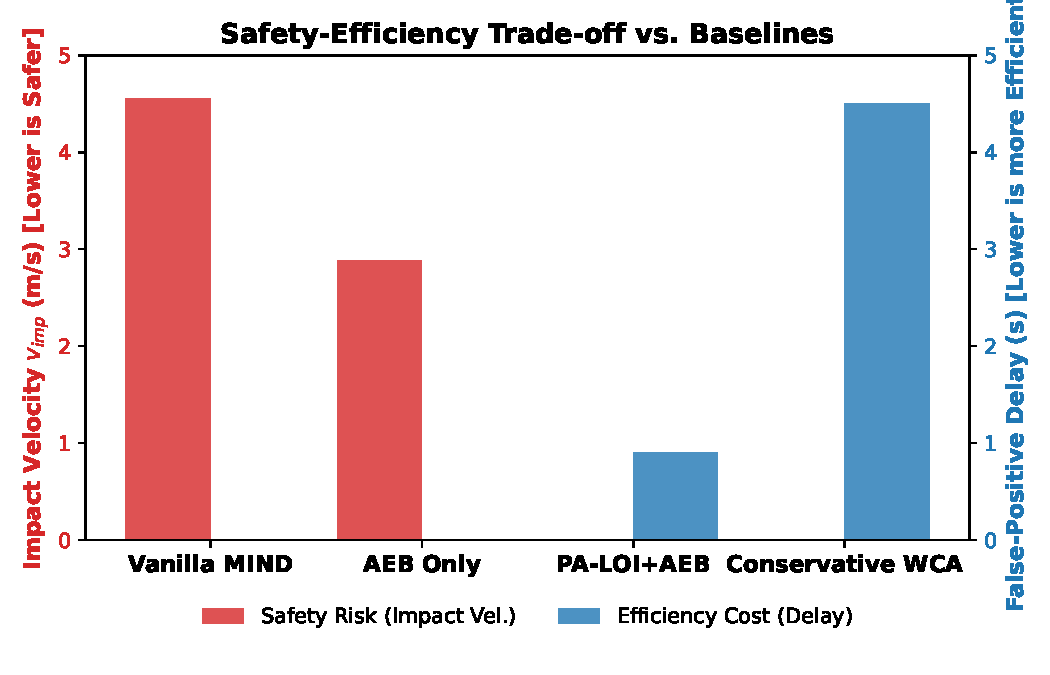
\includegraphics[width=\columnwidth]{figures/pareto_tradeoff.pdf}
\caption{Safety vs. Efficiency trade-off. PA-LOI isolates a Pareto-optimal zone between the unsafe Reactive systems and the highly inefficient WCA (RSS surrogate) baseline.}
\label{fig:pareto}
\end{figure}

% ============================================================
% VI. Discussion
% ============================================================
\section{Discussion}

\subsection{Why Proactive Speed Reduction Matters}
The experimental results reveal a fundamental limitation of reactive AEB: its effectiveness is bounded by the vehicle's kinetic energy at the moment of first detection. In occluded scenarios, the detection-to-collision window is inherently short, making the \emph{approach speed} the decisive factor. PA-LOI addresses this by treating the approach speed itself as a controllable variable, rather than accepting it as a given input to the AEB system.

\subsection{Relationship to Euro NCAP Standards}
Our ghost probe scenario closely mirrors the Euro NCAP CPNA test protocol. The key distinction is that CPNA tests typically use a fixed vehicle speed (e.g., \SI{40}{\kilo\meter\per\hour}), while our scenario allows the planner to determine its own speed profile. This makes the speed at the point of emergence a function of the planning algorithm, which is precisely the variable PA-LOI optimizes.

\subsection{Limitations and Future Work}
While our evaluation covers two geometrically distinct scenarios---a complex intersection and a straight road with dense parked vehicles---additional topologies (e.g., curved roads, multi-lane highways, or T-junctions) remain to be studied. The current risk field relies on map-based geometric occlusion analysis; integrating real-time sensor-based occlusion estimation (e.g., from LiDAR shadow analysis) would improve applicability to unknown environments.

Furthermore, subsequent research will involve integrating PA-LOI with probabilistic tracking modules to evaluate its end-to-end performance in real-world, noisy perception environments and to quantify its impact on large-scale traffic efficiency metrics.

% ============================================================
% VII. Conclusion
% ============================================================
\section{Conclusion}

We presented PA-LOI, a proactive occlusion-aware planning framework that complements reactive AEB systems for pedestrian collision avoidance in ghost probe scenarios. By constructing phantom risk fields around occluded regions and integrating them into trajectory optimization, PA-LOI reduces the ego vehicle's approach speed, thereby extending the effective braking window available to AEB.

Experimental evaluation on two distinct scenarios---a complex intersection and a straight road with dense parked vehicles---demonstrated consistent safety improvements. In the intersection scenario, PA-LOI + AEB achieves zero collision from \SI{2.05}{\meter} clearance versus \SI{3.25}{\meter} for AEB alone (37\% improvement). In the high-speed straight road scenario, AEB alone fails at all tested distances, while PA-LOI + AEB achieves zero collision from just \SI{1.75}{\meter} and reduces worst-case impact velocity by 71\%. These results confirm that proactive, upstream speed management is a critical complement to reactive safety systems in urban autonomous driving.

Future work will extend PA-LOI to additional road topologies, integrate it with sensor-based occlusion estimation~\cite{blindspot2024,occtrack2025}, and evaluate large-scale traffic efficiency impacts.

% ============================================================
% References
% ============================================================
\bibliographystyle{IEEEtran}
\bibliography{references}

\end{document}
